\section{Business Process Modeling Notation (BPMN)}

La información contenida en la actual sección es tomada del libro \textit{BPMN 2.0 Introduction to the Standard for Business Process Modeling} \cite{bpmn2}

A continuación, se enuncian algunos conceptos básicos de BPMN.

\subsection{Enlaces}

Los enlaces sirven para unir o bifurcar el flujo de secuencia de un modelo. Son utilizadas cuando es necesario tomar algún tipo de decisión que lleve a tomar uno o varios caminos alternos. Existen varios tipos de enlaces, como lo son los enlaces exclusivos (XOR), paralelos (AND), inclusivos (OR) y complejos. A continuación, se muestran ejemplos de aplicación de cada uno de estos enlaces.

\begin{figure}[!htb]
  \begin{center}
    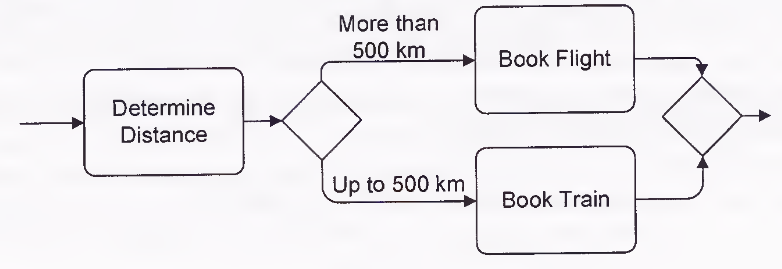
\includegraphics[width=11cm]{./imagenes/gateway_exclusivo.png}
    \caption{Ejemplo de uso del enlace exclusivo}
    \label{fig:gateway_exclusivo}
    \textbf{Fuente:}  \cite{bpmn2}
  \end{center}
\end{figure}

En este caso (Figura \ref{fig:gateway_exclusivo}), se realiza la actividad \textit{Determinar distancia} y se decide que tipo de medio de transporte se debe utilizar. Nótese que luego de realizar la reserva, se vuelve a unir el flujo de secuencia del modelo, ya que no se sabe en la práctica cual de las 2 alternativas será la seleccionada.

\begin{figure}[!htb]
  \begin{center}
    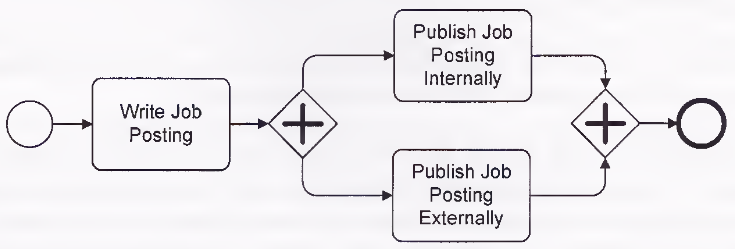
\includegraphics[width=11cm]{./imagenes/gateway_paralelo.png}
    \caption{Ejemplo de uso del enlace paralelo}
    \label{fig:gateway_paralelo}
    \textbf{Fuente:}  \cite{bpmn2}
  \end{center}
\end{figure}

En la figura \ref{fig:gateway_paralelo} se ve un ejemplo de uso de este enlace. Aquí, luego de que se redacta la oferta de trabajo, le procede a publicarla, tanto interna como externamente. En este caso, se utiliza el enlace paralelo para agilizar el proceso de publicación.

\begin{figure}[!htb]
  \begin{center}
    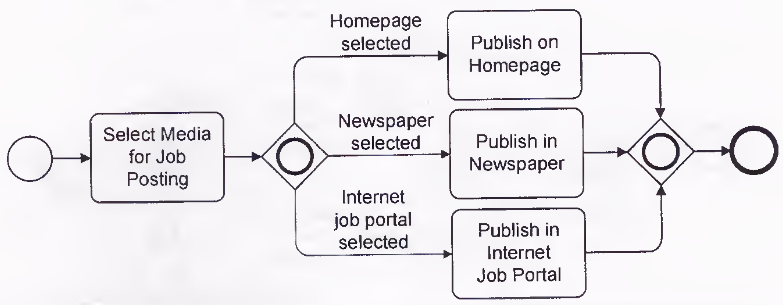
\includegraphics[width=11cm]{./imagenes/gateway_inclusivo.png}
    \caption{Ejemplo de uso del enlace inclusivo}
    \label{fig:gateway_inclusivo}
    \textbf{Fuente:}  \cite{bpmn2}
  \end{center}
\end{figure}


En la figura \ref{fig:gateway_inclusivo} se ve un ejemplo de uso en donde a partir de la actividad ``Seleccionar medio para publicar oferta de trabajo'' se pueden seleccionar una o varias opciones. Cualquier combinación de opciones, que al menos contenga una opción, es válida.

\begin{figure}[!htb]
  \begin{center}
    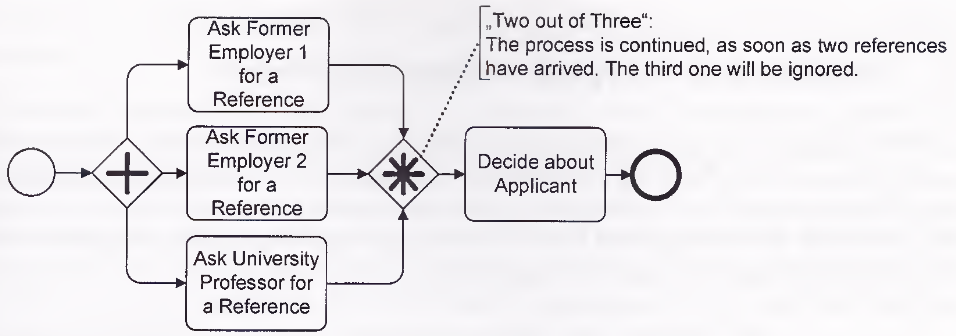
\includegraphics[width=11cm]{./imagenes/gateway_complejo.png}
    \caption{Ejemplo de uso del enlace complejo}
    \label{fig:gateway_complejo}
    \textbf{Fuente:}  \cite{bpmn2}
  \end{center}
\end{figure}


En el ejemplo mostrado en la figura \ref{fig:gateway_complejo}, se requiere la referencia de 2 empleadores previos y de la universidad. En realidad, solo son necesarias dos referencias, pero para estar seguros se piden tres, por lo que tan pronto como llegan las primeras 2 referencias, la tercera puede ser ignorada sin mayor problema.

\subsection{Colaboración}

A menudo, en un proceso intervienen diferentes partes interesadas ({\textit{Stakeholders}) y es necesario ver el proceso de manera global, de manera que el paso de mensajes entre las partes implicadas sea mas claro. A este tipo de diagramas se les llama \textbf{diagrama de colaboración}

La figura \ref{fig:diagrama_colaboracion} muestra como es la interacción entre un aspirante y una empresa en el proceso de acceder a una oferta de empleo. Puede verse como, entre las actividades que ejecuta cada una de las partes, existe un paso de mensaje que une ambos procesos. Esta unión se representa por una flecha con linea punteada, donde un extremo tiene un circulo y el otro una flecha vacía que indica la dirección del mensaje.

\begin{figure}[!htb]
  \begin{center}
    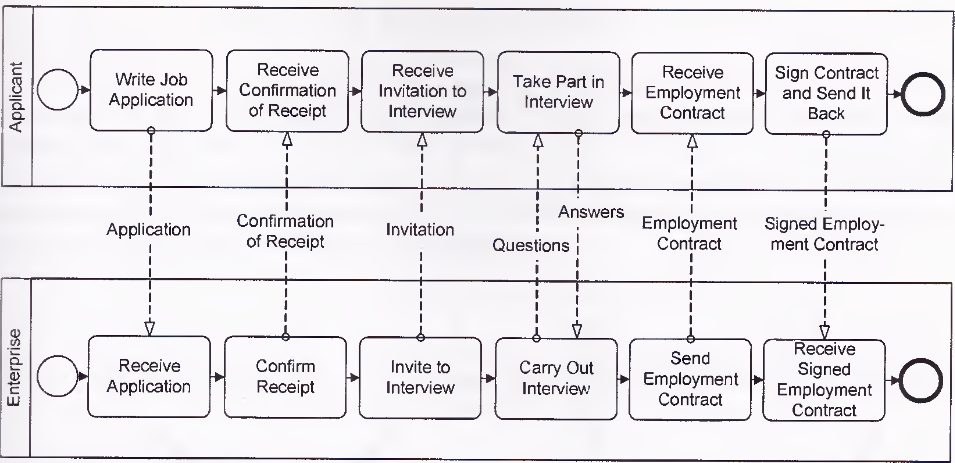
\includegraphics[width=11cm]{./imagenes/diagrama_colaboracion.png}
    \caption{Ejemplo de diagrama de colaboración}
    \label{fig:diagrama_colaboracion}
    \textbf{Fuente:}  \cite{bpmn2}
  \end{center}
\end{figure}


Por ejemplo, la actividad ``Recibir solicitud'' recibe un mensaje de la actividad ``Redactar solicitud de empleo'', por lo cual esta actividad (recibir solicitud) no puede iniciar si el aspirante no envía su solicitud. Esto significa que los mensajes deben ser respetados y una actividad no puede realizarse si le falta algún mensaje de entrada.

Sin embargo, en estos casos solo se conoce el proceso que sigue la empresa, por lo que es común representar a las partes externas como una caja negra (figura \ref{fig:diagrama_colaboracion_caja_negra}).

\begin{figure}[!htb]
  \begin{center}
    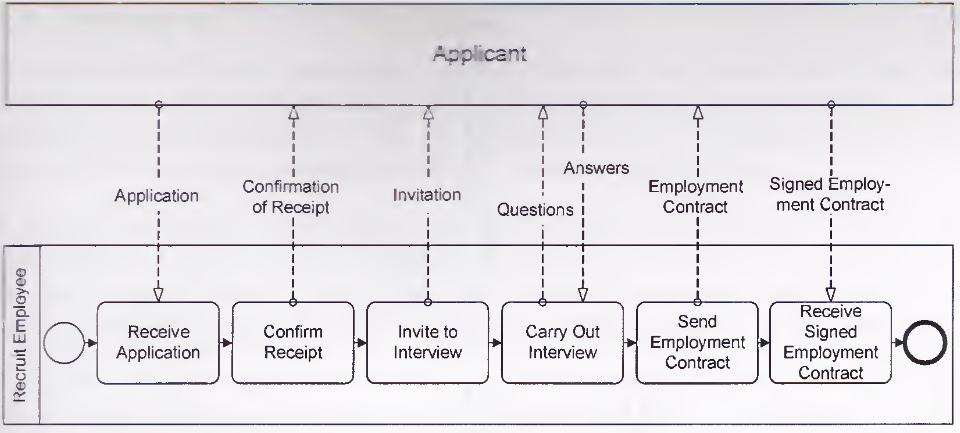
\includegraphics[width=11cm]{./imagenes/diagrama_colaboracion_caja_negra.png}
    \caption{Ejemplo de diagrama de colaboración con caja negra}
    \label{fig:diagrama_colaboracion_caja_negra}
    \textbf{Fuente:}  \cite{bpmn2}
  \end{center}
\end{figure}
